\documentclass[11pt,a4paper]{article}

\usepackage[utf8]{inputenc}
\usepackage[T1]{fontenc}
\usepackage[margin=2.5cm]{geometry}
\usepackage{amsmath}
\usepackage{booktabs}
\usepackage{graphicx}
\usepackage{float}
\usepackage{caption}
\usepackage[hidelinks]{hyperref}

\graphicspath{{figures/}}
\renewcommand{\figurename}{Figura}
\renewcommand{\tablename}{Tabla}
\renewcommand{\refname}{Referencias}
\captionsetup{font=small}
\setlength{\emergencystretch}{2em}

\title{Reporte del Laboratorio 2: Selección de Modelos y Regularización\\
\large Análisis del Dataset: Appliances Energy Prediction}
\author{Oscar Alfonso\\\texttt{of\_alfonso@javeriana.edu.co}
  \and Kevin Bueno\\\texttt{bueno.kevin@javeriana.edu.co}}
\date{26 de septiembre de 2026}

\begin{document}
\maketitle

\section{Contexto de los Datos}

El dataset utilizado se denomina \emph{Appliances Energy Prediction} y proviene del
\emph{UCI Machine Learning Repository} (id 374) \cite{candanedo2017}. Contiene mediciones
tomadas cada 10 minutos durante 4.5 meses (11 de enero al 27 de mayo de 2016) en una vivienda
de bajo consumo en Bélgica. El objetivo es predecir el consumo energético de los
electrodomésticos (\texttt{Appliances}, en Wh) a partir de sensores ambientales.

En los datos encontramos 19\,735 observaciones y 28 predictores:

\begin{itemize}
  \item \textbf{Sensores interiores:} temperatura (\texttt{T1}--\texttt{T9}) y humedad relativa
        (\texttt{RH\_1}--\texttt{RH\_9}) en nueve puntos de la vivienda.
  \item \textbf{Variables meteorológicas exteriores:} temperatura (\texttt{T\_out}), humedad
        (\texttt{RH\_out}), presión (\texttt{Press\_mm\_hg}), viento (\texttt{Windspeed}),
        visibilidad (\texttt{Visibility}) y punto de rocío (\texttt{Tdewpoint}).
  \item \textbf{Otros:} consumo de iluminación (\texttt{lights}) y dos variables aleatorias
        de control (\texttt{rv1}, \texttt{rv2}) introducidas por los autores del dataset.
  \item \textbf{Marca temporal:} \texttt{date}.
\end{itemize}

Los autores del dataset reportan que los modelos con mejor desempeño son de tipo ensamble
(\emph{gradient boosting}, \emph{random forest}) \cite{candanedo2017}, por lo que es esperable
que las regresiones lineales alcancen un poder explicativo modesto. El énfasis de este
laboratorio no es maximizar el desempeño sino aplicar y comparar las técnicas de selección de
modelos y regularización descritas en \cite{islr2023}: \emph{Best Subset Selection},
\emph{Forward} y \emph{Backward Stepwise Selection}, \emph{Ridge}, \emph{Lasso} y
\emph{Principal Components Regression} (PCR).

\section{Exploración de Datos}

\subsection{Calidad de los datos}

El dataset no presenta valores nulos ni filas duplicadas, y los 19\,734 intervalos entre
observaciones consecutivas son exactamente de 10 minutos, es decir, la serie temporal es
continua. La columna \texttt{date} llega como cadena de texto sin separador entre fecha y hora
(por ejemplo, \texttt{2016-01-1117:00:00}), por lo que se parseó con un formato explícito.
Adicionalmente se detectó que \texttt{rv1} y \texttt{rv2} son idénticas; se eliminó
\texttt{rv2} y se conservó \texttt{rv1} como variable de control: al ser ruido aleatorio puro,
un método de selección que funciona correctamente debería descartarla.

\subsection{Variable objetivo}

\begin{table}[H]
  \centering
  \caption{Estadísticas descriptivas de la variable objetivo (\texttt{Appliances}, Wh)}
  \begin{tabular}{lr}
    \toprule
    Métrica & Appliances \\
    \midrule
    count & 19\,735 \\
    mean & 97.69 \\
    std & 102.52 \\
    min & 10 \\
    25\% & 50 \\
    50\% & 60 \\
    75\% & 100 \\
    max & 1\,080 \\
    asimetría (skew) & 3.39 \\
    \bottomrule
  \end{tabular}
\end{table}

La variable objetivo presenta una fuerte asimetría positiva: la media (97.7) supera ampliamente
a la mediana (60) y el 75\% de las observaciones está por debajo de 100 Wh, mientras el máximo
alcanza 1\,080 Wh. Además, los valores están discretizados en saltos de 10 Wh. Dado que la
regresión lineal y sus variantes regularizadas asumen errores aproximadamente simétricos, se
decidió modelar $\log(1 + \texttt{Appliances})$ (ver Figura~\ref{fig:target}).

\begin{figure}[H]
  \centering
  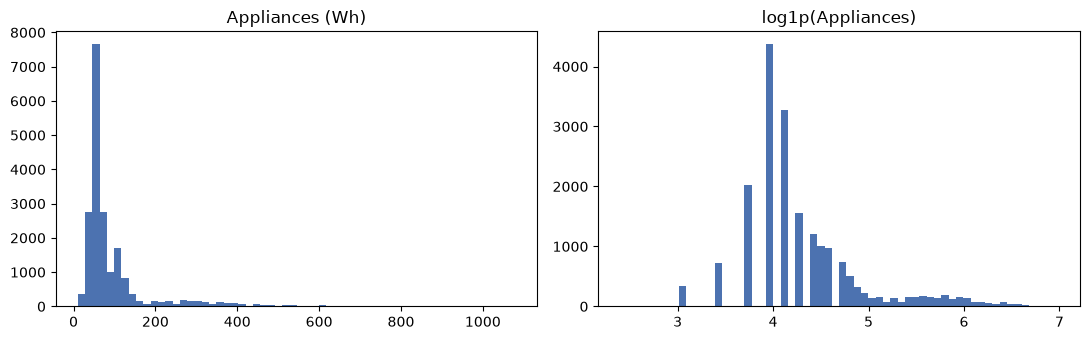
\includegraphics[width=\textwidth]{target_hist.png}
  \caption{Distribución de la variable objetivo en escala original (izquierda) y logarítmica
  (derecha). Los huecos en el histograma logarítmico reflejan la discretización en pasos de 10 Wh.}
  \label{fig:target}
\end{figure}

\subsection{Escala de los predictores}

Los predictores presentan escalas muy heterogéneas (Tabla~\ref{tab:scales}). Como Ridge, Lasso
y PCA son sensibles a la magnitud de las variables, todos los predictores se estandarizaron
(media 0, desviación 1) ajustando el escalador únicamente con el conjunto de entrenamiento.

\begin{table}[H]
  \centering
  \caption{Estadísticas descriptivas de predictores seleccionados (escalas heterogéneas)}
  \label{tab:scales}
  \begin{tabular}{lrrrr}
    \toprule
    Variable & mean & std & min & max \\
    \midrule
    lights & 3.80 & 7.94 & 0.00 & 70.00 \\
    T1 & 21.69 & 1.61 & 16.79 & 26.26 \\
    T6 & 7.91 & 6.09 & $-6.07$ & 28.29 \\
    RH\_6 & 54.61 & 31.15 & 1.00 & 99.90 \\
    T\_out & 7.41 & 5.32 & $-5.00$ & 26.10 \\
    Press\_mm\_hg & 755.52 & 7.40 & 729.30 & 772.30 \\
    RH\_out & 79.75 & 14.90 & 24.00 & 100.00 \\
    rv1 & 24.99 & 14.50 & 0.01 & 50.00 \\
    \bottomrule
  \end{tabular}
\end{table}

La variable \texttt{lights} toma el valor 0 en el 77\% de las observaciones, por lo que se
comporta casi como un indicador binario. Los sensores \texttt{T6} y \texttt{RH\_6}
corresponden a un punto exterior de la vivienda, lo que explica su rango distinto al del resto
de sensores interiores.

\subsection{Análisis de correlaciones}

La matriz de correlación (Figura~\ref{fig:corr}) muestra un patrón de ``tablero de ajedrez'':
todas las temperaturas están fuertemente correlacionadas entre sí, al igual que todas las
humedades. Se trata de una misma vivienda medida en nueve puntos, lo que produce una
multicolinealidad severa. Los pares con $|r| > 0.9$ se listan en la Tabla~\ref{tab:pairs}.

\begin{figure}[H]
  \centering
  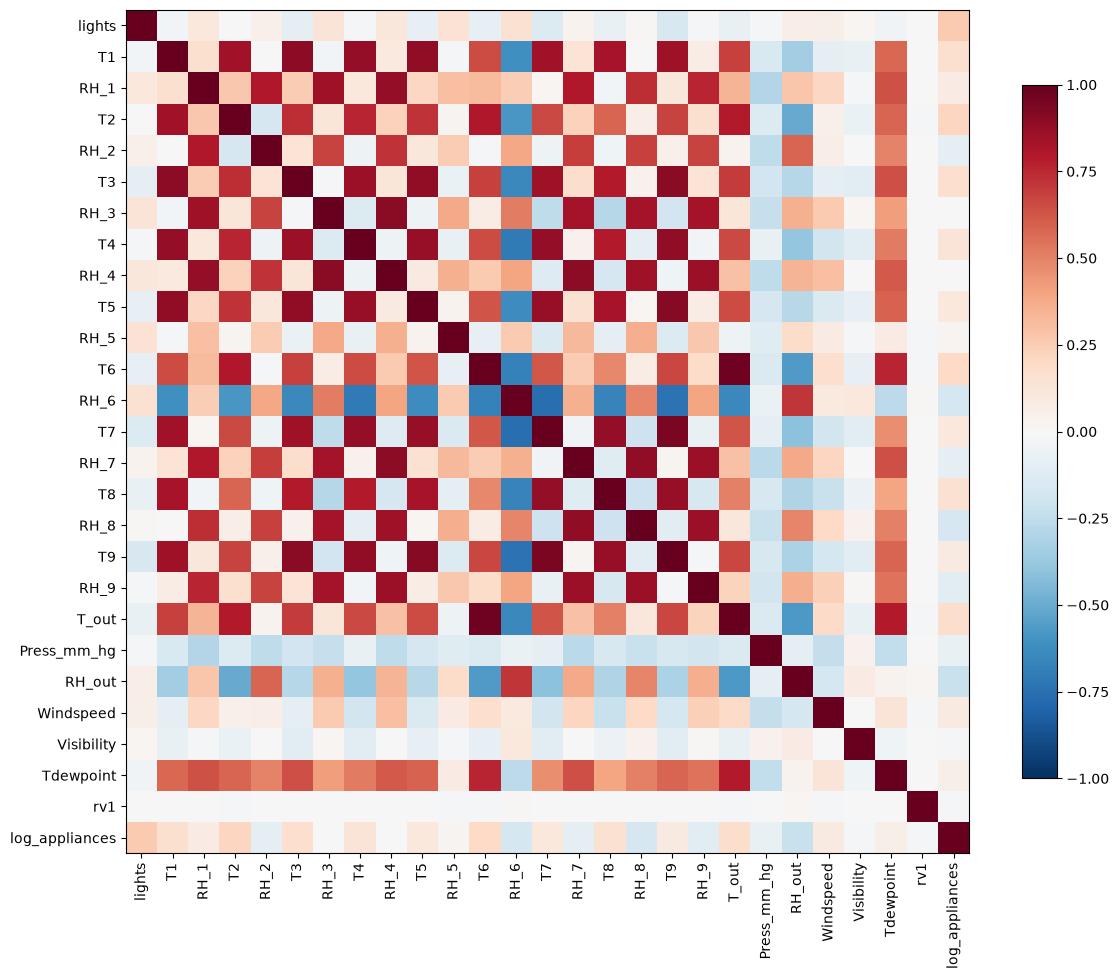
\includegraphics[width=0.85\textwidth]{corr_heatmap.png}
  \caption{Matriz de correlación entre predictores y la variable objetivo transformada.
  La fila de \texttt{rv1} es blanca (correlación nula con todo), como corresponde a ruido aleatorio.}
  \label{fig:corr}
\end{figure}

\begin{table}[H]
  \centering
  \caption{Pares de predictores con correlación absoluta superior a 0.9}
  \label{tab:pairs}
  \begin{tabular}{llr}
    \toprule
    Variable 1 & Variable 2 & $|r|$ \\
    \midrule
    T6 & T\_out & 0.975 \\
    T7 & T9 & 0.945 \\
    T5 & T9 & 0.911 \\
    T3 & T9 & 0.901 \\
    \bottomrule
  \end{tabular}
\end{table}

En contraste, la correlación lineal de los sensores con la variable objetivo es débil: el
máximo corresponde a \texttt{lights} ($r = 0.26$) y ningún sensor de temperatura supera
$r = 0.22$. Se decidió conservar todos los predictores colineales para observar cómo los trata
cada método, en lugar de eliminarlos manualmente.

\subsection{Ingeniería de variables temporales}

Dado que el consumo de electrodomésticos depende de la rutina de los habitantes, se extrajo la
hora del día y el día de la semana de la marca temporal (Figura~\ref{fig:hour}). El consumo
promedio es mínimo en la madrugada, sube a partir de las 7:00 y alcanza su pico a las 18:00.
La hora del día, sin embargo, no debe usarse como entero: las 23:00 y las 0:00 están a una
hora de distancia pero a 23 unidades numéricas. Por ello se codificó de forma cíclica:
\begin{equation}
  \texttt{hour\_sin} = \sin\!\left(\tfrac{2\pi h}{24}\right), \qquad
  \texttt{hour\_cos} = \cos\!\left(\tfrac{2\pi h}{24}\right).
\end{equation}
Estas dos variables alcanzan correlaciones de $-0.35$ y $-0.28$ con el objetivo, superando a
cualquier sensor. El día de la semana resultó irrelevante ($r = 0.02$; el rango de variación
del panel derecho de la Figura~\ref{fig:hour} es de solo 0.17 en escala logarítmica), aunque se
incluyó un indicador \texttt{is\_weekend}. La matriz final contiene 29 predictores.

\begin{figure}[H]
  \centering
  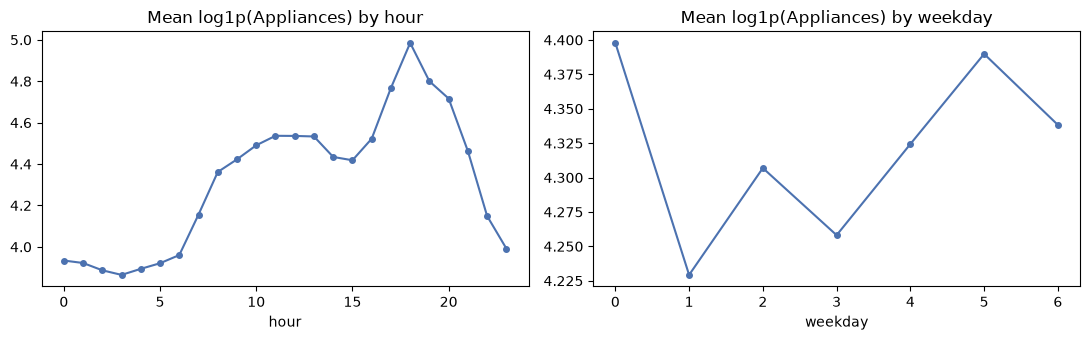
\includegraphics[width=\textwidth]{hour_weekday.png}
  \caption{Consumo promedio (escala logarítmica) por hora del día y por día de la semana.}
  \label{fig:hour}
\end{figure}

\subsection{Partición temporal}

Al tratarse de una serie temporal con observaciones vecinas casi idénticas, una partición
aleatoria produciría fuga de información entre entrenamiento y prueba. Se utilizó una partición
temporal: el primer 80\% de la serie (11 de enero al 30 de abril, 15\,788 filas) para entrenar y
el 20\% restante (30 de abril al 27 de mayo, 3\,947 filas) para probar. Todos los
hiperparámetros ($k$, $\alpha$, $M$) se seleccionaron mediante validación cruzada temporal
(\texttt{TimeSeriesSplit} con 5 particiones) usando únicamente el conjunto de entrenamiento.

\section{Metodología y Análisis de Resultados}

\subsection{Modelo de referencia}

Se ajustó una regresión lineal múltiple con los 29 predictores estandarizados:
\begin{equation}
  \widehat{\log(1+y)} = \beta_0 + \sum_{j=1}^{29} \beta_j X_j.
\end{equation}
Se obtuvo $R^2 = 0.346$ en entrenamiento y $R^2 = 0.229$ en prueba. La brecha entre ambos
refleja un sobreajuste leve y, sobre todo, un cambio de régimen: el modelo se entrena con
invierno e inicios de primavera y se evalúa en mayo, con temperaturas fuera del rango observado.

\subsection{Best Subset Selection}

Con 29 predictores el espacio completo tiene $2^{29} \approx 5.4 \times 10^8$ subconjuntos, lo
que resulta computacionalmente inviable. Se limitó la búsqueda exhaustiva a subconjuntos de
tamaño $k \le 4$ (27\,840 modelos), seleccionando dentro de cada tamaño el subconjunto con mayor
$R^2$ de validación cruzada temporal.

\begin{table}[H]
  \centering
  \caption{Best Subset Selection: mejor subconjunto por tamaño $k$}
  \label{tab:bestsubset}
  \begin{tabular}{clrr}
    \toprule
    $k$ & Predictores & $R^2$ CV & $R^2$ test \\
    \midrule
    1 & hour\_sin & 0.111 & 0.067 \\
    2 & hour\_sin, hour\_cos & 0.194 & 0.179 \\
    3 & T3, hour\_sin, hour\_cos & 0.244 & 0.039 \\
    4 & T3, T6, hour\_sin, hour\_cos & 0.257 & 0.147 \\
    \bottomrule
  \end{tabular}
\end{table}

Dos observaciones destacan. Primero, las variables construidas en el EDA (\texttt{hour\_sin} y
\texttt{hour\_cos}) son las dos primeras seleccionadas entre 29 candidatas. Segundo, el criterio
de validación cruzada sigue mejorando al incluir \texttt{T3}, pero el $R^2$ de prueba se
desploma de 0.179 a 0.039. Para entender este fenómeno se ajustó el modelo con $k = 4$ mediante
\texttt{statsmodels} (Tabla~\ref{tab:ols4}) y se comparó la distribución de \texttt{T3} en
entrenamiento y prueba (Tabla~\ref{tab:t3}).

\begin{table}[H]
  \centering
  \caption{Coeficientes del mejor modelo con $k = 4$ (predictores estandarizados)}
  \label{tab:ols4}
  \begin{tabular}{lrrrr}
    \toprule
    Variable & coef & std err & $t$ & $P>|t|$ \\
    \midrule
    const & 4.3073 & 0.004 & 957.8 & 0.000 \\
    lights & 0.1569 & 0.005 & 33.9 & 0.000 \\
    T3 & 0.1312 & 0.005 & 29.0 & 0.000 \\
    hour\_sin & $-0.1940$ & 0.005 & $-41.8$ & 0.000 \\
    hour\_cos & $-0.1878$ & 0.005 & $-41.7$ & 0.000 \\
    \bottomrule
  \end{tabular}
\end{table}

\begin{table}[H]
  \centering
  \caption{Distribución de \texttt{T3} (°C) en entrenamiento y prueba}
  \label{tab:t3}
  \begin{tabular}{lrr}
    \toprule
    Métrica & train & test \\
    \midrule
    mean & 21.59 & 24.98 \\
    std & 1.50 & 1.39 \\
    25\% & 20.50 & 24.10 \\
    50\% & 21.63 & 24.86 \\
    75\% & 22.60 & 26.17 \\
    \bottomrule
  \end{tabular}
\end{table}

\texttt{T3} es altamente significativa en entrenamiento ($t = 29$, $p < 0.001$), pero el
percentil 25 de \texttt{T3} en prueba (24.1) supera al percentil 75 en entrenamiento (22.6): tres
cuartas partes de las observaciones de mayo caen en una región que el modelo apenas vio. La
relación ``mayor temperatura, mayor consumo'' aprendida en invierno no se sostiene en mayo.
Ni el BIC, ni la validación cruzada temporal, ni la significancia estadística detectan este
problema, porque los tres evalúan dentro del rango de los datos de entrenamiento.

\subsection{Forward y Backward Stepwise Selection}

Se aplicaron ambos procedimientos codiciosos sobre los 29 predictores usando
\texttt{mlxtend}, con el $R^2$ de validación cruzada temporal como criterio en cada paso
(Figura~\ref{fig:stepwise}).

\begin{figure}[H]
  \centering
  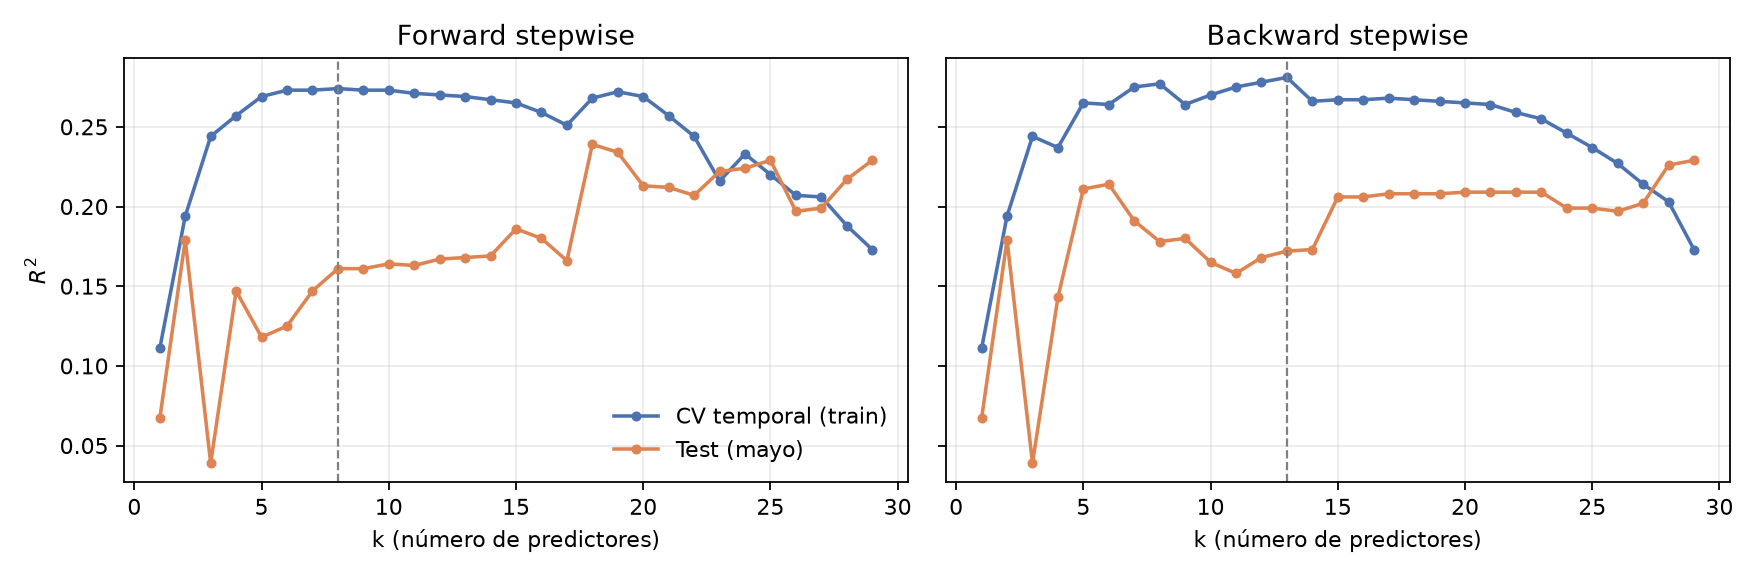
\includegraphics[width=\textwidth]{stepwise_curves.png}
  \caption{$R^2$ de validación cruzada temporal y de prueba en función del número de
  predictores. La línea punteada marca el $k$ óptimo según validación cruzada.}
  \label{fig:stepwise}
\end{figure}

\textbf{Forward.} Los primeros cuatro pasos coinciden exactamente con los ganadores de Best
Subset, de modo que la heurística codiciosa no perdió calidad respecto a la búsqueda exhaustiva.
El $R^2$ de CV alcanza su máximo (0.274) en $k = 8$ con el conjunto \{RH\_1, T3, T5, T6, RH\_9,
Windspeed, hour\_sin, hour\_cos\}. La variable de control \texttt{rv1} ingresa en $k = 9$, es
decir, inmediatamente después de agotarse la señal útil. El $R^2$ de prueba del modelo óptimo es
0.161.

\textbf{Backward.} La primera variable eliminada es \texttt{rv1}. El máximo de CV (0.281)
ocurre en $k = 13$ con un conjunto distinto al de Forward, lo que ilustra que con predictores
intercambiables la selección no es única. El $R^2$ de prueba es 0.172.

Un detalle relevante en la curva de Forward: el $R^2$ de prueba salta de 0.166 a 0.239 en
$k = 18$, cuando ingresa \texttt{T9}, variable con correlaciones superiores a 0.9 con
\texttt{T3}, \texttt{T5} y \texttt{T7}. Sola aporta poco, pero en conjunto con sus pares permite
al modelo aprender \emph{diferencias} entre habitaciones, que son mucho más estables entre
estaciones que las temperaturas absolutas. La multicolinealidad actúa aquí como amortiguador
frente al cambio de régimen.

\subsection{Ridge Regression}

Ridge minimiza $\text{RSS} + \alpha \sum_j \beta_j^2$, encogiendo todos los coeficientes sin
anularlos. El valor $\alpha = 1215$ se seleccionó por validación cruzada temporal sobre una
malla logarítmica de 60 valores. El modelo alcanza $R^2 = 0.332$ en entrenamiento y
$R^2 = 0.242$ en prueba, siendo el único método que supera al modelo de referencia.

\begin{figure}[H]
  \centering
  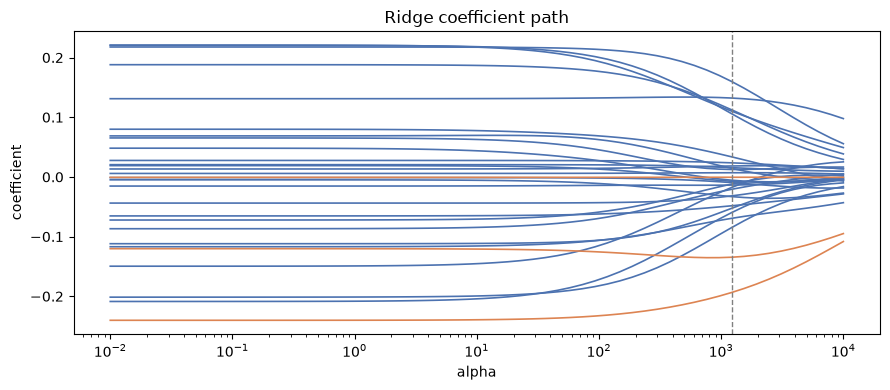
\includegraphics[width=\textwidth]{ridge_path.png}
  \caption{Trayectoria de los coeficientes de Ridge en función de $\alpha$. En naranja,
  \texttt{hour\_sin}, \texttt{hour\_cos} y \texttt{rv1}; la línea punteada marca el $\alpha$ óptimo.}
  \label{fig:ridge}
\end{figure}

En la Figura~\ref{fig:ridge} se observa que los pares colineales (\texttt{T6}/\texttt{T\_out},
\texttt{T7}/\texttt{T9}) reciben en OLS coeficientes grandes de signo opuesto que se cancelan
mutuamente, firma clásica de la multicolinealidad; Ridge los aplasta a partir de $\alpha \approx
100$. Las variables horarias son las últimas en encogerse, y \texttt{rv1} permanece pegada a
cero en todo el recorrido.

\subsection{Lasso Regression}

Lasso minimiza $\text{RSS} + \alpha \sum_j |\beta_j|$, lo que produce coeficientes exactamente
nulos y por tanto selección automática de variables. Con $\alpha = 0.012$ (validación cruzada
temporal), el modelo conserva 17 de los 29 predictores (Tabla~\ref{tab:lasso}) y anula
\texttt{rv1}. Obtiene $R^2 = 0.315$ en entrenamiento y $R^2 = 0.213$ en prueba.

\begin{table}[H]
  \centering
  \caption{Coeficientes no nulos de Lasso, ordenados por magnitud}
  \label{tab:lasso}
  \begin{tabular}{lr@{\hspace{2cm}}lr}
    \toprule
    Variable & coef & Variable & coef \\
    \midrule
    hour\_cos & $-0.200$ & RH\_7 & $-0.022$ \\
    hour\_sin & $-0.161$ & RH\_8 & $-0.020$ \\
    T3 & 0.141 & T4 & $-0.011$ \\
    lights & 0.135 & RH\_5 & 0.010 \\
    T8 & 0.086 & is\_weekend & 0.008 \\
    T9 & $-0.072$ & Press\_mm\_hg & $-0.006$ \\
    RH\_1 & 0.038 & T\_out & $-0.002$ \\
    RH\_3 & 0.034 & & \\
    RH\_9 & $-0.031$ & & \\
    T6 & $-0.030$ & & \\
    \bottomrule
  \end{tabular}
\end{table}

\begin{figure}[H]
  \centering
  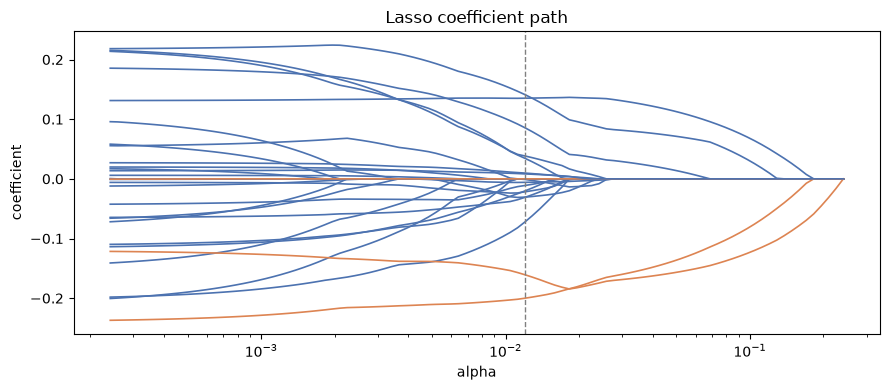
\includegraphics[width=\textwidth]{lasso_path.png}
  \caption{Trayectoria de los coeficientes de Lasso. Leída de derecha a izquierda, el orden de
  ingreso es \texttt{hour\_sin}, \texttt{hour\_cos}, \texttt{T3}, \texttt{lights}: el mismo que
  encontraron Best Subset y Forward.}
  \label{fig:lasso}
\end{figure}

Lasso pierde frente al modelo de referencia por la misma razón que los métodos Stepwise:
elimina precisamente los sensores redundantes (\texttt{T5}, \texttt{T7}, \texttt{T\_out}) que
estabilizan la extrapolación, mientras conserva \texttt{T3} con un coeficiente elevado.

\subsection{Análisis de Componentes Principales y PCR}

PCA construye combinaciones lineales de los predictores ordenadas por varianza explicada. Se
requieren 8, 12 y 15 componentes para explicar el 80\%, 90\% y 95\% de la varianza
(Figura~\ref{fig:scree}), confirmando la redundancia entre sensores. Sobre estas componentes se
ajustó una regresión lineal (PCR), eligiendo el número de componentes $M$ por validación
cruzada temporal (Figura~\ref{fig:pcr}).

\begin{figure}[H]
  \centering
  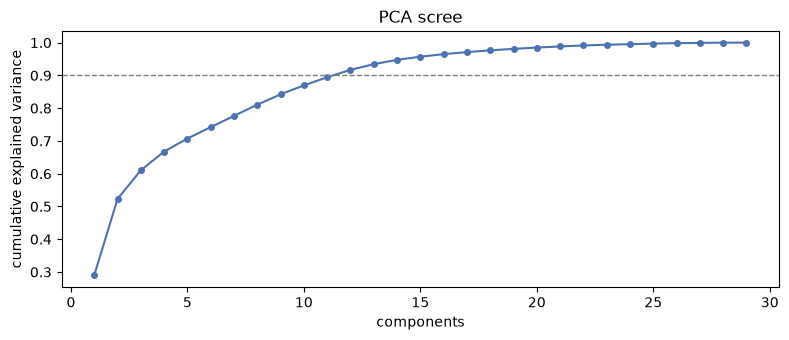
\includegraphics[width=0.8\textwidth]{pca_scree.png}
  \caption{Varianza explicada acumulada por componente principal.}
  \label{fig:scree}
\end{figure}

\begin{figure}[H]
  \centering
  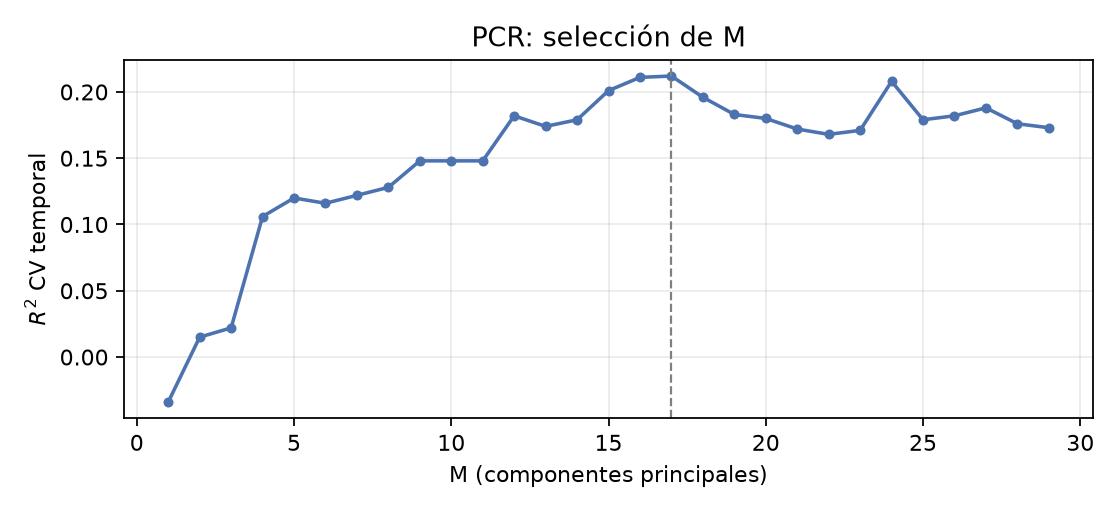
\includegraphics[width=0.7\textwidth]{pcr_cv.png}
  \caption{$R^2$ de validación cruzada temporal de PCR en función de $M$.}
  \label{fig:pcr}
\end{figure}

El resultado más ilustrativo es que las tres primeras componentes, que explican el 61\% de la
varianza de los predictores, tienen un $R^2$ de CV prácticamente nulo. Los saltos en $M = 4$ y
$M = 12$ corresponden al ingreso de las componentes que cargan sobre \texttt{hour\_sin} y
\texttt{hour\_cos}. PCA es no supervisado: maximiza la varianza de $X$ sin mirar $y$, y la
varianza dominante vive en los sensores redundantes mientras la señal predictiva vive en dos
columnas de baja varianza compartida. Se requirieron $M = 17$ componentes para alcanzar
$R^2 = 0.227$ en prueba, sin mejora respecto a la regresión con los 29 predictores originales.

\section{Comparación de Modelos}

\begin{table}[H]
  \centering
  \caption{Comparación de los modelos ajustados (partición temporal, objetivo $\log(1+y)$)}
  \label{tab:final}
  \begin{tabular}{lrrrr}
    \toprule
    Modelo & Predictores & $R^2$ train & $R^2$ test & RMSE test \\
    \midrule
    Ridge ($\alpha = 1215$) & 29 & 0.332 & \textbf{0.242} & 0.487 \\
    OLS (todos los predictores) & 29 & 0.346 & 0.229 & 0.491 \\
    PCR ($M = 17$) & 17 & 0.310 & 0.227 & 0.491 \\
    Lasso ($\alpha = 0.012$) & 17 & 0.315 & 0.213 & 0.496 \\
    Best Subset ($k = 2$) & 2 & 0.200 & 0.179 & 0.506 \\
    Backward Stepwise ($k = 13$) & 13 & 0.304 & 0.172 & 0.508 \\
    Best Subset ($k = 3$) & 3 & 0.248 & 0.163 & 0.511 \\
    Forward Stepwise ($k = 8$) & 8 & 0.265 & 0.161 & 0.512 \\
    Best Subset ($k = 4$) & 4 & 0.286 & 0.081 & 0.536 \\
    Best Subset ($k = 1$) & 1 & 0.130 & 0.067 & 0.540 \\
    \bottomrule
  \end{tabular}
\end{table}

La Tabla~\ref{tab:final} muestra un gradiente claro: los métodos que conservan todos los
predictores (Ridge, OLS, PCR) ocupan los primeros lugares; Lasso, que elimina con moderación,
queda en el medio; y los métodos de selección agresiva (Best Subset, Stepwise) ocupan los
últimos. Cuantas más variables se eliminan, peor es la extrapolación a mayo.

\section{Conclusiones}

\begin{enumerate}
  \item Ridge es el único método que supera al modelo de referencia en prueba ($R^2 = 0.242$
        frente a $0.229$). Encoger los coeficientes sin eliminar predictores resulta la
        estrategia adecuada cuando los predictores redundantes amortiguan un cambio de
        distribución.
  \item Todos los métodos que eliminan variables (Best Subset, Forward, Backward, Lasso) mejoran
        el $R^2$ de validación cruzada pero empeoran el de prueba respecto a la referencia. Los
        sensores colineales que descartan son los que estabilizan la extrapolación a un periodo
        más cálido.
  \item Ningún criterio in-sample (BIC, validación cruzada temporal, significancia estadística)
        detectó que \texttt{T3} extrapola mal. La validación cruzada protege contra el
        sobreajuste al ruido, pero no contra un futuro cuya distribución difiere del pasado.
  \item La señal más robusta es la hora del día, construida en el EDA mediante codificación
        cíclica. Cuatro algoritmos independientes (Best Subset, Forward, Backward y Lasso) la
        seleccionaron en primer lugar entre 29 candidatas.
  \item La variable de control \texttt{rv1} fue descartada por los seis métodos: Lasso la anuló,
        Backward la eliminó primero, Forward la incorporó solo tras agotar la señal útil, y
        Ridge la mantuvo pegada a cero.
  \item PCR no aporta mejoras: la varianza dominante de los predictores corresponde a sensores
        redundantes, mientras la señal predictiva reside en direcciones de baja varianza.
  \item Limitaciones: Best Subset se truncó en $k \le 4$ por costo computacional, y el $R^2$
        absoluto es bajo en todos los casos porque el consumo depende de comportamientos de los
        habitantes que los sensores no capturan, en línea con lo reportado en
        \cite{candanedo2017}.
\end{enumerate}

\appendix
\section{Código fuente}

El código completo del laboratorio (carga de datos, EDA, ingeniería de variables, los seis
métodos y la tabla comparativa) se encuentra en el notebook \texttt{notebooks/lab02.ipynb} del
siguiente repositorio:

\begin{center}
  \url{https://github.com/aristotekean/ml-lab02-best-subset-lasso}
\end{center}

\begin{thebibliography}{9}
  \bibitem{islr2023} James, G., Witten, D., Hastie, T., \& Tibshirani, R. (2023).
    \emph{An Introduction to Statistical Learning: with Applications in R} (2nd ed.). Springer.
    \url{https://www.statlearning.com/}
  \bibitem{candanedo2017} Candanedo, L. M., Feldheim, V., \& Deramaix, D. (2017).
    Data driven prediction models of energy use of appliances in a low-energy house.
    \emph{Energy and Buildings}, 140, 81--97.
\end{thebibliography}

\end{document}
